\documentclass[review]{siamart171218}
\usepackage[utf8]{inputenc}
\usepackage[english]{babel}

\usepackage{tikz}
\usetikzlibrary{shapes.geometric}
\usetikzlibrary{plotmarks}
\usetikzlibrary{arrows.meta}

\usepackage{pgfplots}
\pgfplotsset{compat=newest}
\usepgfplotslibrary{patchplots}

\usepackage{algorithm}
\usepackage{algorithmicx}
\usepackage[noend]{algpseudocode}
\usepackage{amsfonts}
\usepackage{amsmath}
\usepackage{amssymb}
\usepackage{amsthm}
\usepackage[title]{appendix}
\usepackage{bm}
\usepackage{booktabs}
\usepackage{cite}
\usepackage{dsfont}
\usepackage{enumitem}
\usepackage{fancyhdr}
\usepackage{graphicx}
\usepackage{grffile}
\usepackage{import}
\usepackage{mathrsfs}
\usepackage{mathtools}
\usepackage{microtype}
\usepackage{overpic}
\usepackage{refcheck}
\usepackage{stmaryrd}
\usepackage{varwidth}
\usepackage{xcolor}

\DeclareMathOperator*{\argmax}{arg\,max}
\DeclareMathOperator*{\argmin}{arg\,min}
\DeclarePairedDelimiter\ceil{\lceil}{\rceil}
\DeclarePairedDelimiter\floor{\lfloor}{\rfloor}

\renewcommand{\vec}[1]{\bm{#1}}
\newcommand{\R}[0]{\mathbb{R}}
\newcommand{\C}[0]{\mathbb{C}}
\newcommand{\ttrank}{{\rm rank}^{\rm TT}}
\newcommand{\mlrank}{{\rm rank}^{\rm ML}}
\newcommand{\cprank}{{\rm rank}^{\rm CP}}
\newcommand{\rank}{{\rm rank}}
\newcommand{\lex}{<_{\rm lex}}
\newcommand{\lexeq}{\le_{\rm lex}}

%\theoremstyle{definition}
%\newtheorem{definition}{Definition}[section]
%\newtheorem{theorem}{Theorem}[section]
%\newtheorem{corollary}{Corollary}[theorem]
%\newtheorem{lemma}[theorem]{Lemma}
\newtheorem{example}{Example}[section]

\graphicspath{{figures/}}
\makeatletter
\def\input@path{{figures/}}
\makeatother

\title{The ultraspherical spectral element method\thanks{Submitted to the editors \today.
\funding{This work is supported by National Science Foundation grant no.~1818757 and the National Defense Science and Engineering Graduate Fellowship.}}}
\author{Daniel Fortunato\thanks{School of Engineering and Applied Sciences, Harvard University, Cambridge, MA 02138. (\email{dfortunato@g.harvard.edu})} \and Nicholas Hale\thanks{Department of Mathematical Sciences, Stellenbosch University, Stellenbosch, 7602, South Africa. (\email{nickhale@sun.ac.za})} \and Alex Townsend\thanks{Department of Mathematics, Cornell University, Ithaca, NY 14853. (\email{townsend@cornell.edu})}}
\headers{ultraSEM}{Daniel Fortunato, Nicholas Hale, and Alex Townsend}
\begin{document}
\maketitle

\begin{abstract}
We introduce a novel spectral element method based on the ultraspherical spectral method and the hierarchical Poincare--Steklov scheme for solving general partial differential equations (PDEs) on polygonal unstructured meshes.  Properties of the ultraspherical spectral method lead to almost banded well-conditioned linear systems, allowing for the element method to be competitive in the ultra-high-polynomial regime and to be robust to meshes that contain elements with small aspect ratios. The hierarchical Poincare--Steklov scheme enables precomputed solution operators to be reused, allowing for fast elliptic solves in implicit and semi-implicit time-steppers. We develop an open-source software system...
\end{abstract}

\begin{keywords}
spectral element method, ultraspherical spectral method, hierarchical Poincare--Steklov scheme
\end{keywords}

\begin{AMS}
65N35, 65N55, 65M60
\end{AMS}

\section{Introduction}\label{sec:introduction}
%{\bf Advantages}
%\begin{enumerate}
%\item Complexity is $\mathcal{O}(p^4/h^3)$ instead of $\mathcal{O}(p^6/h^3)$.
%\item Closer to ``true" $hp$-adaptivity, since this allows for $p$ in the hundreds.
%\item Stability?
%\item Robust to skinny elements.
%\item Storage of solution operator allows for fast solves with multiple RHSs/BCs (e.g. time-stepping).
%\item Hierarchical Poincar\'{e}--Steklov can be used as an element method (i.e. it doesn't have to look like nested dissection).
%\item No mapping between grids to deal with corners.
%\end{enumerate}

Traditional approaches for solving partial differential equations (PDEs) include finite element, finite differences, and spectral element methods. Each approach represents the sought-after PDE solution on a grid or mesh. Convergence is then achieved by shrinking the grid or mesh spacing. 

Traditional approaches have several drawbacks in the spectral element methods: (1) Iterative solvers are not necessarily robust because of the difficult in designing preconditioners; 
(2) The numerics are sensitive to elements with a small aspect ratio; (3) They are restricted to relatively small polynomial degrees ($<15$) because of dense linear algebra; and (4) An algorithmic complexity that makes the high $p$ regime computationally expensive. In this paper, we propose a variant on a hierarchical Poincare--Steklov scheme that employs the utlraspherical spectral method instead of collocation. At its heart, we derive a coefficient-based 




 
Current spectral element methods have a large computational complexity and numerical instability when employing high degree polynomials on each element. This means that $h$-refinement in $hp$-adaptivity is usually preferred over $p$-adaptivity, introspective of local error estimators. Here, we take advantage of the recent advances in spectral methods, to propose a spectral element method with a numerical stability that is independent of the polynomial degrees employed and a computational complexity of $\mathcal{O}()$. We believe this alleviates the current computational burden on mesh generation software and begins to make the high-$p$ regime competitive. In particular, we are able to represent solutions with piecewise polynomials of degrees in the hundreds or even thousands. 


For spectral element methods based on the pseudospectral method the overall complexity is $\mathcal{O}(Np^4 + N^{3/2})$, where $N \approx (p/h)^2$ is the total number of degrees of freedom, $p$ is the polynomial degree on each element, and $h$ is the average mesh element size. This  severely restricts the competitiveness of the high $p$ regime in $hp$-adaptivity (for high $p$ the complexity is $\mathcal{O}(N^3)$) and makes $h$-refinement preferred over $p$-adaptivity. It is important to alleviate this restriction so that $hp$-adaptivity can be entirely based on local error estimators. Ideally, the complexity should only depend on $N$.

We go some way to achieving this goal by developing a Hierarchical Poincare--Steklov scheme that costs:
\[
 \underbrace{\frac{p^4}{h^2}}_{\text{leaf computation}} + \underbrace{\frac{p^3}{h^3}}_{\text{merge cost}} + \underbrace{\frac{p^2}{h} + \frac{p}{h}\log \frac{p}{h}}_{\text{solve cost}} \approx \frac{p^4}{h^2} + \frac{p^3}{h^3} \approx Np^2 + N^{3/2}. 
\]

\begin{figure}[htb]
  \centering
  \begin{minipage}{0.49\textwidth}
    \begin{center}
      \small
      \scalebox{0.4}{% This file was created by matlab2tikz.
%
%The latest updates can be retrieved from
%  http://www.mathworks.com/matlabcentral/fileexchange/22022-matlab2tikz-matlab2tikz
%where you can also make suggestions and rate matlab2tikz.
%
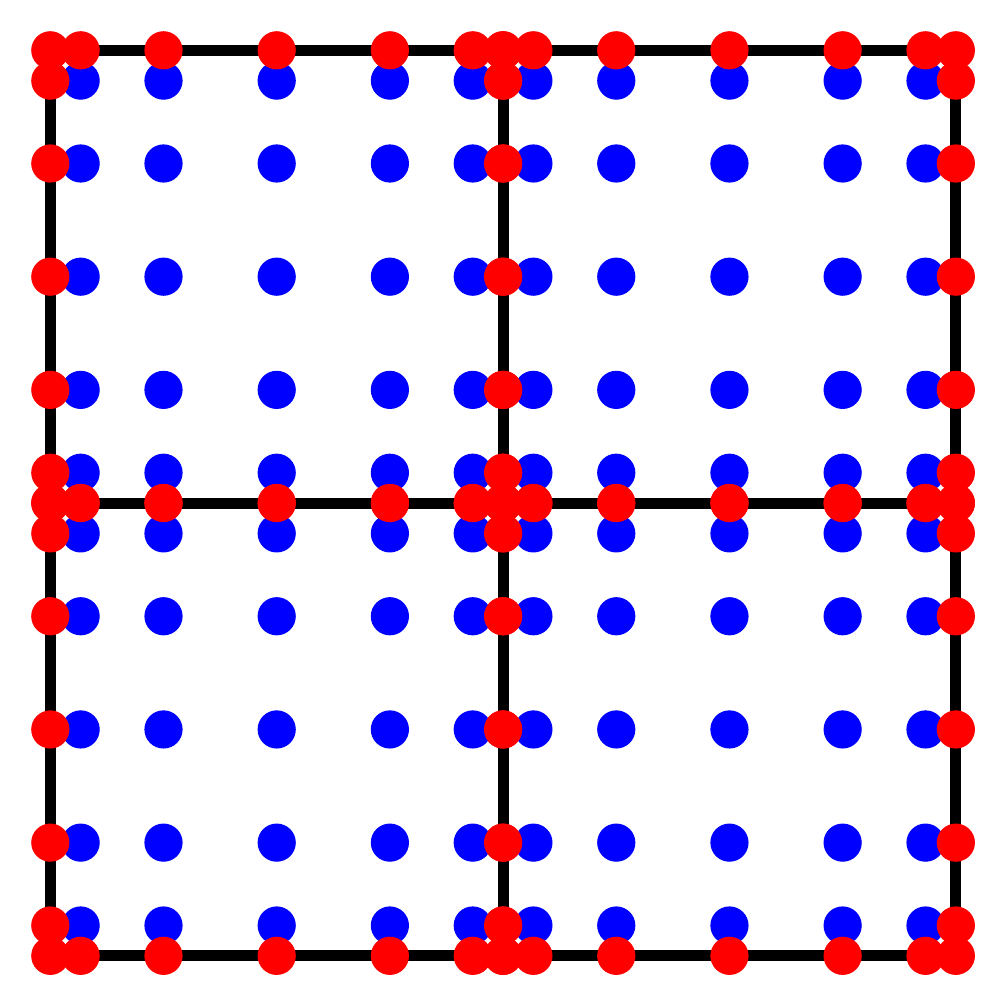
\begin{tikzpicture}

\begin{axis}[%
width=4.754in,
height=4.754in,
at={(1.648in,0.642in)},
scale only axis,
xmin=-2.1,
xmax=2.1,
ymin=-2.1,
ymax=2.1,
axis line style={draw=none},
ticks=none,
axis x line*=bottom,
axis y line*=left
]
\draw[line width=4.0pt, draw=black] (axis cs:0,0) rectangle (axis cs:2,2);
\addplot [color=blue, only marks, mark size=6.7pt, mark=*, mark options={solid, blue}, forget plot]
  table[row sep=crcr]{%
0.133974596215561	0.133974596215561\\
0.133974596215561	0.5\\
0.133974596215561	1\\
0.133974596215561	1.5\\
0.133974596215561	1.86602540378444\\
0.5	0.133974596215561\\
0.5	0.5\\
0.5	1\\
0.5	1.5\\
0.5	1.86602540378444\\
1	0.133974596215561\\
1	0.5\\
1	1\\
1	1.5\\
1	1.86602540378444\\
1.5	0.133974596215561\\
1.5	0.5\\
1.5	1\\
1.5	1.5\\
1.5	1.86602540378444\\
1.86602540378444	0.133974596215561\\
1.86602540378444	0.5\\
1.86602540378444	1\\
1.86602540378444	1.5\\
1.86602540378444	1.86602540378444\\
};
\addplot [color=red, only marks, mark size=6.7pt, mark=*, mark options={solid, red}, forget plot]
  table[row sep=crcr]{%
0	0\\
0	0.133974596215561\\
0	0.5\\
0	1\\
0	1.5\\
0	1.86602540378444\\
0	2\\
0.133974596215561	0\\
0.133974596215561	2\\
0.5	0\\
0.5	2\\
1	0\\
1	2\\
1.5	0\\
1.5	2\\
1.86602540378444	0\\
1.86602540378444	2\\
2	0\\
2	0.133974596215561\\
2	0.5\\
2	1\\
2	1.5\\
2	1.86602540378444\\
2	2\\
};
\draw[line width=4.0pt, draw=black] (axis cs:-2,0) rectangle (axis cs:0,2);
\addplot [color=blue, only marks, mark size=6.7pt, mark=*, mark options={solid, blue}, forget plot]
  table[row sep=crcr]{%
-1.86602540378444	0.133974596215561\\
-1.86602540378444	0.5\\
-1.86602540378444	1\\
-1.86602540378444	1.5\\
-1.86602540378444	1.86602540378444\\
-1.5	0.133974596215561\\
-1.5	0.5\\
-1.5	1\\
-1.5	1.5\\
-1.5	1.86602540378444\\
-1	0.133974596215561\\
-1	0.5\\
-1	1\\
-1	1.5\\
-1	1.86602540378444\\
-0.5	0.133974596215561\\
-0.5	0.5\\
-0.5	1\\
-0.5	1.5\\
-0.5	1.86602540378444\\
-0.133974596215561	0.133974596215561\\
-0.133974596215561	0.5\\
-0.133974596215561	1\\
-0.133974596215561	1.5\\
-0.133974596215561	1.86602540378444\\
};
\addplot [color=red, only marks, mark size=6.7pt, mark=*, mark options={solid, red}, forget plot]
  table[row sep=crcr]{%
-2	0\\
-2	0.133974596215561\\
-2	0.5\\
-2	1\\
-2	1.5\\
-2	1.86602540378444\\
-2	2\\
-1.86602540378444	0\\
-1.86602540378444	2\\
-1.5	0\\
-1.5	2\\
-1	0\\
-1	2\\
-0.5	0\\
-0.5	2\\
-0.133974596215561	0\\
-0.133974596215561	2\\
0	0\\
0	0.133974596215561\\
0	0.5\\
0	1\\
0	1.5\\
0	1.86602540378444\\
0	2\\
};
\draw[line width=4.0pt, draw=black] (axis cs:0,-2) rectangle (axis cs:2,0);
\addplot [color=blue, only marks, mark size=6.7pt, mark=*, mark options={solid, blue}, forget plot]
  table[row sep=crcr]{%
0.133974596215561	-1.86602540378444\\
0.133974596215561	-1.5\\
0.133974596215561	-1\\
0.133974596215561	-0.5\\
0.133974596215561	-0.133974596215561\\
0.5	-1.86602540378444\\
0.5	-1.5\\
0.5	-1\\
0.5	-0.5\\
0.5	-0.133974596215561\\
1	-1.86602540378444\\
1	-1.5\\
1	-1\\
1	-0.5\\
1	-0.133974596215561\\
1.5	-1.86602540378444\\
1.5	-1.5\\
1.5	-1\\
1.5	-0.5\\
1.5	-0.133974596215561\\
1.86602540378444	-1.86602540378444\\
1.86602540378444	-1.5\\
1.86602540378444	-1\\
1.86602540378444	-0.5\\
1.86602540378444	-0.133974596215561\\
};
\addplot [color=red, only marks, mark size=6.7pt, mark=*, mark options={solid, red}, forget plot]
  table[row sep=crcr]{%
0	-2\\
0	-1.86602540378444\\
0	-1.5\\
0	-1\\
0	-0.5\\
0	-0.133974596215561\\
0	0\\
0.133974596215561	-2\\
0.133974596215561	0\\
0.5	-2\\
0.5	0\\
1	-2\\
1	0\\
1.5	-2\\
1.5	0\\
1.86602540378444	-2\\
1.86602540378444	0\\
2	-2\\
2	-1.86602540378444\\
2	-1.5\\
2	-1\\
2	-0.5\\
2	-0.133974596215561\\
2	0\\
};
\draw[line width=4.0pt, draw=black] (axis cs:-2,-2) rectangle (axis cs:0,0);
\addplot [color=blue, only marks, mark size=6.7pt, mark=*, mark options={solid, blue}, forget plot]
  table[row sep=crcr]{%
-1.86602540378444	-1.86602540378444\\
-1.86602540378444	-1.5\\
-1.86602540378444	-1\\
-1.86602540378444	-0.5\\
-1.86602540378444	-0.133974596215561\\
-1.5	-1.86602540378444\\
-1.5	-1.5\\
-1.5	-1\\
-1.5	-0.5\\
-1.5	-0.133974596215561\\
-1	-1.86602540378444\\
-1	-1.5\\
-1	-1\\
-1	-0.5\\
-1	-0.133974596215561\\
-0.5	-1.86602540378444\\
-0.5	-1.5\\
-0.5	-1\\
-0.5	-0.5\\
-0.5	-0.133974596215561\\
-0.133974596215561	-1.86602540378444\\
-0.133974596215561	-1.5\\
-0.133974596215561	-1\\
-0.133974596215561	-0.5\\
-0.133974596215561	-0.133974596215561\\
};
\addplot [color=red, only marks, mark size=6.7pt, mark=*, mark options={solid, red}, forget plot]
  table[row sep=crcr]
    \end{center}
  \end{minipage}%
  \begin{minipage}{0.49\textwidth}
    \begin{center}
      \small
      \scalebox{0.42}{% This file was created by matlab2tikz.
%
%The latest updates can be retrieved from
%  http://www.mathworks.com/matlabcentral/fileexchange/22022-matlab2tikz-matlab2tikz
%where you can also make suggestions and rate matlab2tikz.
%
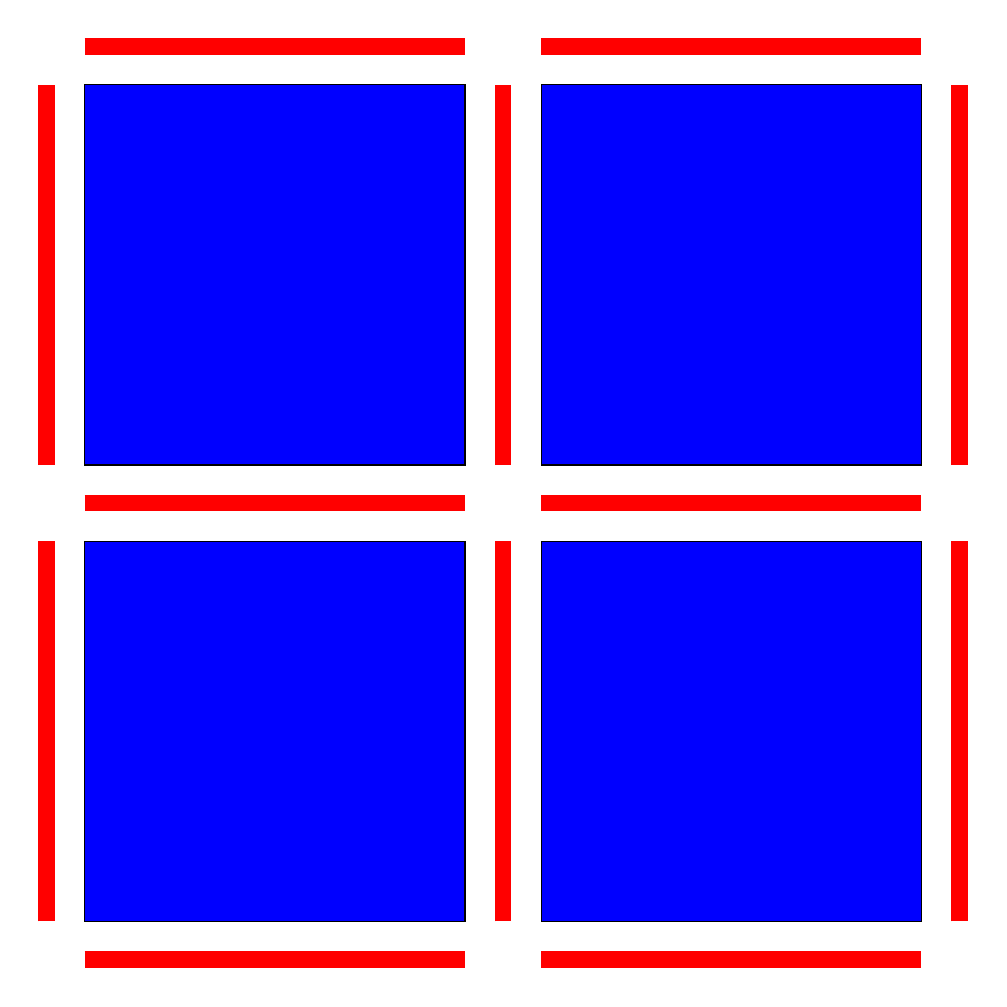
\begin{tikzpicture}

\begin{axis}[%
width=4.754in,
height=4.754in,
at={(1.648in,0.642in)},
scale only axis,
xmin=-2.5,
xmax=2.5,
ymin=-2.5,
ymax=2.5,
axis line style={draw=none},
ticks=none,
axis x line*=bottom,
axis y line*=left
]
\draw[fill=blue, draw=black] (axis cs:0.2,0.2) rectangle (axis cs:2.2,2.2);
\draw[fill=blue, draw=black] (axis cs:-2.2,0.2) rectangle (axis cs:-0.2,2.2);
\draw[fill=blue, draw=black] (axis cs:0.2,-2.2) rectangle (axis cs:2.2,-0.2);
\draw[fill=blue, draw=black] (axis cs:-2.2,-2.2) rectangle (axis cs:-0.2,-0.2);
\addplot [color=red, line width=6.0pt, forget plot]
  table[row sep=crcr]{%
0	0.2\\
0	2.2\\
};
\addplot [color=red, line width=6.0pt, forget plot]
  table[row sep=crcr]{%
0	-2.2\\
0	-0.2\\
};
\addplot [color=red, line width=6.0pt, forget plot]
  table[row sep=crcr]{%
-2.2	0\\
-0.2	0\\
};
\addplot [color=red, line width=6.0pt, forget plot]
  table[row sep=crcr]{%
0.2	0\\
2.2	0\\
};
\addplot [color=red, line width=6.0pt, forget plot]
  table[row sep=crcr]{%
2.4	0.2\\
2.4	2.2\\
};
\addplot [color=red, line width=6.0pt, forget plot]
  table[row sep=crcr]{%
2.4	-2.2\\
2.4	-0.2\\
};
\addplot [color=red, line width=6.0pt, forget plot]
  table[row sep=crcr]{%
-2.4	0.2\\
-2.4	2.2\\
};
\addplot [color=red, line width=6.0pt, forget plot]
  table[row sep=crcr]{%
-2.4	-2.2\\
-2.4	-0.2\\
};
\addplot [color=red, line width=6.0pt, forget plot]
  table[row sep=crcr]{%
-2.2	2.4\\
-0.2	2.4\\
};
\addplot [color=red, line width=6.0pt, forget plot]
  table[row sep=crcr]{%
0.2	2.4\\
2.2	2.4\\
};
\addplot [color=red, line width=6.0pt, forget plot]
  table[row sep=crcr]{%
-2.2	-2.4\\
-0.2	-2.4\\
};
\addplot [color=red, line width=6.0pt, forget plot]
  table[row sep=crcr]
    \end{center}
  \end{minipage}
  \vspace{1em}
  \caption{Two interpretations of domain decomposition using the Schur complement method, with interface data in red and interior data in blue. (Left) In value space, neighboring elements communicate directly through shared degrees of freedom, which can be partitioned into shared interface nodes and local interior nodes. (Right) Neighboring elements communicate indirectly through unshared interface unknowns, allowing for domain decomposition that is independent of basis.}
  \label{fig:dd_interpretations}
\end{figure}

\section{Background material}\label{sec:background}
First, we describe the fundamental ideas in the ultraspherical spectral method~\cite{Olver_13_01}, which in one dimension solves linear ordinary differential equations (ODEs) with variable coefficients of the form: 
\[
\sum_{j=0}^M a_j(x)\frac{d^ju}{dx^j} = f(x), \quad x\in[-1,1], \qquad \mathcal{B}u = c, 
\]
where $\mathcal{B}u=c$ are general linear boundary (such as Dirichlet) or interior conditions to ensure that there is a unique solution. For an integer $p$ the method seeks to compute the first $p$ Chebyshev expansion coefficients $\{u_j\}_{j=0}^{p-1}$ of the solution $u$, where $u(x) = \sum_{j=0}^\infty u_j T_j(x)$ and $T_j(x) = \cos(j\cos^{-1}x)$ is the degree $j$ Chebyshev polynomial (of the first kind). 

The spectral method, at its most simplest, is based on the following recurrence relationships~\cite[(18.9.21) \& (18.9.9)]{NISTHandbook}: 
\[
 \frac{d}{dx} T_j(x) = jU_{j-1}(x), \quad j\geq 1, \qquad T_j(x) = \frac{1}{2}\left(U_{j}(x)-U_{j-2}(x)\right), \quad j\geq 2,
\]
where $U_{j}(x) = \sin((j+1)\cos^{-1}x)/\sin(\cos^{-1}x)$ is the degree $j$ Chebyshev polynomial of the second kind. This means that differentiation and basis conversion can be represented by the following (extremely) sparse operators:
\[
 \mathcal{D}_1 = \begin{pmatrix}0 & 1 \cr &&2\cr &&&3\cr &&&&\ddots\cr & \end{pmatrix}, \qquad \mathcal{S}_0 = \frac{1}{2}\begin{pmatrix}2 & 0 &-1\cr & 1 & 0 & -1 \cr && 1 & 0 & \ddots\cr &&& 1 &\ddots\cr &&&&\ddots  \end{pmatrix}.  
\]
These operators can be combined to represent first-order linear ordinary differential operators, for example, $u'(x) + u(x)$ becomes $\mathcal{D}_1 + \mathcal{S}_0$, where the solution is represented in modes of the first kind basis and the range in modes of the second kind basis. 

The operator $\mathcal{D}_1 + \mathcal{S}_0$ has just three nonzero superdiagonals, constructing --- albeit, for a very simple example --- a sparse and spectrally accurate representation of a differential operator.  This is in stark contrast to pseudospectral methods or tau methods that lead to dense linear systems.  

The first-order ODE given by $u'(x)+a(x)u(x)$ requires an operator to represent multiplication by $a(x)$, denoted by $\mathcal{M}[a]$. If $a(x)$ is a degree $m$ polynomial the operator $\mathcal{M}[a]$ is a $m$-banded and is aToeplitz-plus-Hankel-plus-rank-1 operator~\cite{Olver_13_01}. The ultraspherical representation $\mathcal{D}_1 + \mathcal{S}_0\mathcal{M}[a]$ has a bandwidth of $m+2$. 

Higher order differentiation remains sparse by exploiting a hierarchy of bases known as ultraspherical polynomials. They satisfy the following recurrence relations~\cite[(18.9.19),(18.9.7)]{NISTHandbook}:
\[
 \frac{d}{dx}C_j^{(\lambda)}(x) = 2\lambda C_{j-1}^{(\lambda+1)},\quad n\geq 1, \qquad (j+\lambda)C_j^{(\lambda)}(x) = \lambda\left(C_{j}^{(\lambda+1)}(x) -C_{j-2}^{(\lambda+1)}(x)\right), \quad j\geq 2,
\]
where $C^{(\lambda)}_j$ is the degree $j$ ultraspherical polynomial with parameter $\lambda$ and $U_j = C^{(1)}_j$. Moreover, multiplication operators for a degree $m$ polynomial are also $m$ banded and can be explicitly constructed~\cite{Olver_13_01}. All this means that linear differential operators of any differential order (with variable coefficients that are well-approximated by polynomials) can be represented with banded operators, where the solution is represented in modes of the Chebyshev basis and the range in modes of the $C^{(M)}$. Here, $M$ is the differential order of the ODE. 

Figure~\ref{fig:JacobiPlane} (left) shows the so-called {\em Jacobi plane}. The position of an orthogonal polynomial basis depends on the weight function, $w(x) = (1-x)^\alpha(1+x)^\beta$, with respect to which it is an orthogonal basis.  It is a remarkable fact that simple recurrence relations for differentiation and basis conversion exist between integer spaced sets of Jacobi polynomials. The ultraspherical spectral method exploits this to derive banded representations of 1D linear differential operators. 

\begin{figure}
 \centering 
 \begin{minipage}{.49\textwidth}
   \centering
  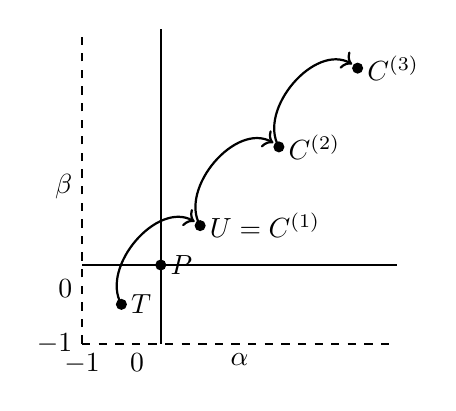
\begin{tikzpicture}
  \draw[black,dashed,thick] (0,0) -- (0,4);
  \draw[black,dashed,thick] (0,0) -- (4,0);
  \draw[black,thick] (1,0) -- (1,4);
  \draw[black,thick] (0,1) -- (4,1);
  \node[anchor=north] at (2,0) (xaxis) {$\alpha$};
  \node[anchor=east] at (0,2) (yaxis) {$\beta$};
  \node[anchor=north] at (0,0) (m1) {$-1$};
  \node[anchor=east] at (0,0) (m1) {$-1$};
  \node[anchor=north] at (.7,0) (m1) {$0$};
  \node[anchor=east] at (0,.7) (m1) {$0$};
  \fill (.5,.5) circle[radius=2pt];
  \fill (1.5,1.5) circle[radius=2pt];
  \fill (1,1) circle[radius=2pt];
  \fill (2.5,2.5) circle[radius=2pt];
  \fill (3.5,3.5) circle[radius=2pt];
  \node[anchor=west] at (1,1) (Legendre) {$P$};
  \node[anchor=west] at (.5,.5) (ChebyshevT) {$T$};
  \node[anchor=west] at (1.5,1.5) (ChebyshevU) {$U=C^{(1)}$};
  \node[anchor=west] at (2.5,2.5) (UltraS2) {$C^{(2)}$};
  \node[anchor=west] at (3.5,3.5) (UltraS3) {$C^{(3)}$};
  \draw[thick] (ChebyshevT.west) edge[out=120,in=150,->] (1.43,1.55);
  \draw[thick] (ChebyshevU.west) edge[out=120,in=150,->] (2.43,2.55);
  \draw[thick] (UltraS2.west) edge[out=120,in=150,->] (3.43,3.55);
  \end{tikzpicture}
  \end{minipage}
\begin{minipage}{.49\textwidth}
\includegraphics[width=\textwidth]{simpleboundarylayer}
\end{minipage}
  \caption{Left: Jacobi plane. Jacobi polynomials $P^{(\alpha,\beta)}$ are orthogonal polynomials associated with the weight function $w(x) = (1-x)^\alpha(1+x)^\beta$, $\alpha,\beta>-1$. Sparse recurrence relations for differentiation and basis conversion exist between bases $C^{(\lambda)}$ and $C^{(\lambda+1)}$, indicated by the black arrows. Along the diagonal $\alpha=\beta>-1/2$ the orthogonal polynomials are referred to as {\em ultraspherical polynomials} and are denoted by $C^{(\lambda)}$. Right: The solution of $\epsilon u''(x) + xu'(x)+\sin(x)u(x) = 0$, $u(\pm 1) = 1$, for $\epsilon = 10^{-1}, 10^{-3}, 10^{-7}$. The ultraspherical spectral method typically constructs well-conditioned banded matrices and can compute solutions with extremely high polynomial degree. Here for $\epsilon=10^{-7}$, a Chebyshev expansion of degree $22,\!950$ is required to resolve the boundary layer of width $\mathcal{O}(\epsilon)$ to $15$ digits.}
  \label{fig:JacobiPlane}
\end{figure}

The ultraspherical spectral method must also impose boundary conditions. This is achieved by {\em boundary bordering}, i.e., the last few rows of the resulting linear system are replaced by rows (usually dense) that impose the constraint on the Chebyshev coefficients of the solution. The resulting linear system has a distinctive {\em almost banded} structure (banded with a few dense boundary rows). A specialized adaptive QR routine has been developed for adaptively generating and solving linear systems with this structure~\cite{Olver_13_01}. If the solution is well-approximated by a Chebyshev expansion of degree $p$, then the ODE solution is  computed in $\mathcal{O}(m^2p)$ operations. The technique of boundary bordering allows the ultraspherical spectral method to automatically and conveniently deal with general linear boundary or interior conditions. Boundary bordering is not structure preserving but is an essential part of delivering the flexibility required by many users. The ultraspherical spectral method is implemented in Chebfun~\cite{Chebfun}, which is a software system for numerical computations with functions and differential equations.  

The constructed linear systems are provably well-conditioned in a precise sense~\cite[Lem.~4.4]{Olver_13_01} and hence, can typically be solved to an accuracy close to machine precision. Moreover, the differential and basis conversion operators contain entries that are exactly representable in floating point arithmetic and extensive numerical experimentation has shown that the ultraspherical spectral method can accurately solve difficult singularly perturbed differential equations, see Figure~\ref{fig:JacobiPlane} (right). This is the crucial 
numerical feature for deriving a spectral element method that is not sensitive to small aspect ratios.

\subsection{The ultraspherical spectral method for linear PDEs defined on rectangular domains}\label{sec:rectangularDomains}
The ultraspherical spectral method can be extended to two dimensions, which can be more efficient than na\"{i}ve Kronecker products~\cite{Townsend_15_01} and computes modes of the solution in the bivariate tensor product Chebyshev basis.  It is based on separable models of linear partial differential operators. That is, any linear differential operator in two variables, $\mathfrak{L}$, can be written as a sum of tensor-products of differential operators in one variable as follows:
\begin{equation}
\mathfrak{L} = \sum_{j=1}^k \left(\mathfrak{L}_j^y\otimes \mathfrak{L}_j^x\right),
\label{eq:separableModel}
\end{equation}
where $\mathfrak{L}^y_1,\ldots, \mathfrak{L}^y_k$ are operators associated to ODEs in $y$ and $\mathfrak{L}_1^x,\ldots, \mathfrak{L}_k^x$ are operators associated to ODEs in $x$.
The {\em splitting rank} of $\mathfrak{L}$ is the minimum number of terms in such a representation.  A separable model gives us a scheme for discretizing PDEs since the individual univariate differential operators $\mathfrak{L}^y_1,\ldots, \mathfrak{L}^y_k, \mathfrak{L}_1^x,\ldots, \mathfrak{L}_k^x$ can be discretized using the ultraspherical spectral method.  Calculating the representation in~\eqref{eq:separableModel} is especially useful for discretizing PDEs in an automatic way and is now the method of choice for the direct PDE solver in Chebfun~\cite{Chebfun,Townsend_15_01}.

When the splitting rank is $2$ a discretization of the PDE is a generalized Sylvester matrix equation that can be solved with special linear algebra techniques costing only $\mathcal{O}(N^{3/2})$ operations, where $N$ is the number of modes used to represent the solution. When the splitting rank is $>2$ the discretization is expanded into a squared-times larger linear system using Kronecker products. The almost banded structure of the ultraspherical discretizations means that resulting linear system is block banded with a few dense boundary rows and can be solved in $\mathcal{O}(N^2)$ operations.

\section{The ultraspherical hierarchical Poincare--Steklov scheme for two elements}
Explanation of our Poincare--Steklov scheme for two squares. 

\section{The ultraspherical hierarchical Poincare--Steklov scheme for multiple elements}
Explanation of our Poincare--Steklov scheme for multiple merges. 

\section{Mesh elements with small aspect ratios}
For solving PDEs on geometries with pinching boundaries elements with small aspect ratios are inevitable. These types of geometries are common in airfoil simulations since the airfoil ends abruptly. These simulations involve high-advection fluid flow so it should be a setting where spectral element methods are very competitive.  I will exploit the properties 
of the ultraspherical spectral method for solving singularly perturbed differential equations to analyze why the spectral method proposed can accurately solve problems even when elements have small aspect ratios.

\section*{Acknowledgements}

\nocite{*}
\bibliographystyle{siamplain}
\bibliography{references}

\end{document}